% intro:
    % partiti da implementazione seriale per avere baseline per confronto di performance
    % implementata prima versione parallela CUDA 
    % miglioramento versione parallela con rappresentazione BCSR
    % versione migliore con workbalance e approccio vertex centric

% versione seriale
    % pseudo codice
        % global relabel (euristica)
        
% prima versione parallela
    % pseudo codice
    % cooperative groups (perché? senza c'era cattiva sincronizzazione tra threads)
    % tentativi di miglioramento con mem pagelocked e mapped mem
    % dati rappresentati con matrice di adiacenza
    % test -> troppa memoria utilizzata 


% rappresentazione CSR (e BCSR) [Appendice B?]

% miglioramento prima versione con rappresentazione BCSR
    % inserire confronti di pezzi di codice tra le due versioni

% versione workbalanced con approccio vertex centric
    % problema risolto: prima ogni thread si occupava di un solo nodo (se nodo non attivo, thread "sprecato")
    % ora: prima si cercano i nodi attivi e poi si suddividono i thread in gruppi e ognuno si occupa di un nodo
    % approccio ideato da [paper]
    % pseudo codice
    
% parallelizzaione findMinCutSet con OpenMP

% dati in input
    % random graphs (generazione)
    % DIMACS
    % funzioni per la lettura

% test condotti
    % per variazione di numero di nodi (a densità costante)
    % per variazione di densità (a  numero di nodi costante)
    % su istanze verosimili (DIMACS)
    % misurazione dei tempi
    % salvataggio risultati
    % calcolo tempi medi 

\chapter{Implementazione e ottimizzazioni}

    In questo capitolo presentiamo il percorso seguito per lo sviluppo di diverse versioni di un algoritmo parallelo per il calcolo del taglio minimo in un grafo. Il punto di partenza è stato l'implementazione di un algoritmo seriale, utilizzato come baseline per il confronto delle performance. Successivamente, si è passati a una prima versione parallela basata su CUDA, con l'obiettivo di sfruttare il calcolo parallelo per migliorare l'efficienza.

    Dopo questa prima versione, è stato introdotto un miglioramento significativo attraverso l'uso della rappresentazione BCSR (Bidirectional Compressed Sparse Row), ottimizzata per ridurre il consumo di memoria e migliorare l'accesso ai dati. A seguire, ulteriori ottimizzazioni sono state implementate tramite un approccio work-balanced e vertex-centric, che hanno risolto il problema della scarsa efficienza dei thread inattivi, migliorando il bilanciamento del carico di lavoro tra i thread attivi. Questo approccio è stato proposto da un recente studio \cite{EngineeringWorkload2024} e si è dimostrato efficace nel massimizzare l'utilizzo delle risorse hardware.
    
    Infine, vengono presentati i dettagli dei test eseguiti utilizzando grafi generati casualmente e dataset standard in formato DIMACS. I test hanno valutato le prestazioni delle implementazioni in funzione del numero di nodi e della densità dei grafi, con un'analisi dettagliata dei tempi di esecuzione.


    \section{Versione seriale}

        La prima versione dell'algoritmo push-relabel implementata è stata quella seriale. Il codice sviluppato segue passo passo lo pseudocodice riportato nel Capitolo \ref{chap:DescrizioneProblema}.
        Le performance misurate sono apparse sin da subito scarse con tempi che crescevano esponenzialmente all'aumentare del numero di nodi del grafo in input.

        Le cause di questi risultati sono riconducibili in buona parte all'elevato numero di operazioni di relabel, molte delle quali inutili. 
        Per ovviare al problema, Goldberg e Tarjan hanno proposto un'euristica chiamata \textit{global relabeling} \cite{PushRelabel} che impedisce all'altezza dei nodi di aumentare velocemente e assegna ai nodi la minor altezza possibile.

        La tecnica di global relabeling prevede l'esecuzione di una Breadth First Search (BFS) all'indietro (partendo dal nodo sink) nel grafo residuo, assegnando ai nodi nuove altezze corrispondenti al livello di ciascun nodo nell'albero BFS. La BFS richiede un tempo lineare pari a $O(m + n)$. In genere, il global relabeling viene applicato una volta ogni $n$ operazioni di relabel. Questa euristica migliora notevolmente le prestazioni dell'algoritmo push-relabel.

        Questa euristica, riportata nell'Algoritmo \ref{alg:global-relabel}, è stata implementata in tutte le versioni parallele che verranno descritte in seguito in questo capitolo.

        \begin{algorithm}
            \caption{Euristica \textit{Global Relabeling}}\label{alg:global-relabel}
            \begin{algorithmic}
                \State make queue $Q$ empty 
                \ForAll{$v \in V$}
                    \State $scanned[v] \gets false$
                \EndFor
                \State $Q.$push($t$)
                \State $scanned[t] \gets true$
                \While{$Q \neq \emptyset $}
                    \State $x \gets Q.$pop()
                    \State $current \gets h(x)$
                    \State $current \gets current + 1$
                    \ForAll{$(y,x) \in E_f : y $ not scanned}
                        \State $h(y) \gets current$
                        \State $scanned[y] \gets true$
                        \State $Q.$pop()
                    \EndFor     
                \EndWhile
            \end{algorithmic}
        \end{algorithm}


    \section{Prima versione parallela}

        Nella versione parallelizzata dell'algoritmo push-relabel si assume che il numero di thread in esecuzione sia |V| e che ciascuno di essi gestisca esattamente un nodo del grafo, comprese tutte le operazioni di push e relabel su di esso. In alcuni casi, più nodi possono essere gestiti da un solo thread.

        Sia $x$ il thread in esecuzione che rappresenta il nodo $x \in V$. Ogni thread ha i seguenti attributi privati: 
        \begin{itemize}
        \item la variabile $e'$ che memorizza l'eccesso del nodo $x$;
        \item la variabile $h''$ che memorizza l'altezza del vicino $y$ di $x$ tale che $(x, y) \in E_f$;
        \item la variabile $h'$ che memorizza l'altezza del vicino $y'$ di $x$ con altezza minore.
        \end{itemize}
        
        Altre variabili sono condivise tra tutti i thread in esecuzione. Tra queste ci sono gli array che contengono gli eccessi ($e$) e le altezze dei nodi ($h$), le capacità residue degli archi ($c_f$) e una variabile $TotalExcess$ equivalente al valore del flusso uscente dal nodo sorgente.

        Tutti i thread in esecuzione hanno accesso alle variabili nella memoria globale, ma i loro compiti vengono eseguiti sequenzialmente grazie all'accesso atomico ai dati. L'ordine delle operazioni in questa sequenza non può essere previsto. Nonostante ciò, l'algoritmo può essere dimostrato corretto.

        Inizialmente, l'operazione di inizializzazione ($Init$) viene eseguita dall'host (Algoritmo \ref{alg:parallel-init}). Questo codice di inizializzazione è lo stesso della versione seriale dell'algoritmo push-relabel.
        
        Il corpo principale dell'algoritmo è controllato dall'host. Il thread host esegue un ciclo \verb|while| fino a quando il valore cumulativo degli eccessi memorizzati nella sorgente e nel pozzo raggiunge il valore di $TotalExcess$ (Algoritmo \ref{alg:parallel-main}). A questo punto, tutto il flusso valido arriva al pozzo, mentre il resto del flusso torna alla sorgente. Di conseguenza, l'eccesso nel pozzo è uguale al valore del flusso massimo.

        Nel primo passo del ciclo \verb|while|, il thread host copia le altezze dei nodi nel device e avvia il kernel push-relabel. Quando il controllo ritorna al thread host, il "flusso" calcolato e le altezze dei nodi vengono copiati nella memoria della CPU e viene eseguita l'operazione di global-relabel. 
        
        Nel kernel push-relabel (Algoritmo \ref{alg:parallel-pr-kernel}), per $CYCLE$ iterazioni (dove $CYCLE$ è una costante che abbiamo definito pari a $|V|$), il thread cerca il nodo vicino con altezza minore verso cui effettuare un'operazione di push o di relabel. 
        Il ciclo \verb|while| nel kernel, quindi, si interrompe dopo un numero di iterazioni definito da $CYCLE$ e non quando il suo nodo diventa inattivo.  

        Al momento dell'esecuzione del global-relabeling (Algoritmo \ref{alg:parallel-global-relabel}), poiché il ciclo \verb|while| del kernel può terminare in qualsiasi momento, può verificarsi che la proprietà di alcuni archi residui $(x, y) \in E_f$ venga violata, cioè $h(x) > h(y) + 1$. Pertanto, prima di calcolare le nuove altezze dei nodi con il global-relabeling, tutti gli archi che violano la proprietà vengono corretti tramite il push del flusso. Gli eccessi dei nodi che non sono raggiungibili dalla BFS all'indietro devono essere sottratti da $TotalExcess$ poiché rappresentano un eccesso accumulato che non raggiungerà mai il pozzo.

        
        \begin{algorithm}
            \caption{\textit{Init()}}\label{alg:parallel-init}
            \begin{algorithmic}
                \State $h(s) \gets |V|$
                \State $e(s) \gets 0$
                \ForAll{$(u,y) \in E$}
                    \State $c_f(x,y) \gets c_{xy}$
                    \State $c_f(y,x) \gets c_{yx}$
                \EndFor
                \ForAll{$(s,x) \in E$}
                    \State $c_f(s,x) \gets 0$
                    \State $c_f(x,s) \gets c_{xs} + c_{sx}$
                    \State $e(s) \gets c_{sx}$
                    \State $TotalExcess \gets TotalExcess + c_{sx}$
                \EndFor
            \end{algorithmic}
        \end{algorithm}

        \begin{algorithm}
            \caption{\textit{PushRelabelKernel()}}\label{alg:parallel-pr-kernel}
            \begin{algorithmic}
                \State $cycle =$ CYCLE
                \While{$cycle > 0$}
                    \If{$e(x) > 0$ and $h(x) < |V|$}
                        \State $e' \gets e(x)$
                        \State $h' \gets \infty$
                        \ForAll{$(x,y) \in E_f$}
                            \State $h'' \gets h(y)$
                            \If{$h'' < h'$}
                                \State $y' \gets y$
                                \State $h' \gets h''$
                            \EndIf
                        \EndFor
                        \If{$h(x) > h'$} \qquad \Comment{Thread performs PUSH}
                            \State $\delta \gets min\{e', c_f(x,y)\}$
                            \State AtomicAdd($c_f(y',x), \delta$)
                            \State AtomicSub($c_f(x,y'), \delta$)
                            \State AtomicAdd($e(y'), \delta$)
                            \State AtomicSub($e(x), \delta$)
                        \Else \qquad \Comment{Thread performs RELABEL}
                            \State $h(u) \gets h' + 1$
                        \EndIf
                    \EndIf
                    \State $cycle = cycle - 1$
                \EndWhile
            \end{algorithmic}
        \end{algorithm}
    
        \begin{algorithm}
            \caption{\textit{GlobalRelabel()}}\label{alg:parallel-global-relabel}
            \begin{algorithmic}
                \ForAll{$(x,y) \in E$}
                    \If{$h(x) > h(y) + 1$}
                        \State $e(x) \gets e(x) - c_f(x,y)$
                        \State $e(y) \gets e(y) + c_f(x,y)$
                        \State $c_f(y,x) \gets c_f(y,x) + c_f(x,y)$
                        \State $c_f(x,y) \gets 0$
                    \EndIf
                \EndFor
                \State do a backwards BFS from sink and assign the height function with each node’s BFS tree level
                \If{not all the nodes are scanned}
                    \ForAll{$x \in V$}
                        \If{$x$ is not scanned and not marked}
                            \State mark $x$
                            \State $TotalExcess \gets TotalExcess - e(x)$
                        \EndIf
                    \EndFor
                \EndIf
            \end{algorithmic}
        \end{algorithm}

        \begin{algorithm}
            \caption{\textit{Main()}}\label{alg:parallel-main}
            \begin{algorithmic}
                \State \textit{Init()}
                \State Copy $e$ and $c_f$ from the CPU's main memory to the CUDA device global memory
                \While{$e(s)+e(t) < TotalExcess$}
                    \State Copy $h$ from the CPU's main memory to the CUDA device global memory
                    \State \textit{PushRelabelKernel()}
                    \State Copy $e$, $c_f$ and $h$ from the CUDA device global memory to the CPU's main memory
                    \State \textit{GlobalRelabel()}
                \EndWhile
            \end{algorithmic}
        \end{algorithm}


        \subsection{Implementazione kernel Push-Relabel}

            \textbf{Nota:} tutti i nomi di funzioni che seguiranno fanno riferimento al codice consegnato.
            
            La funzione host \verb|pushRelabel| gestisce l'intero processo dell'algoritmo, eseguendo i seguenti passaggi:
            \begin{itemize}
                \item preflow iniziale dai nodi sorgente;
                \item trasferimento delle variabili necessarie sulla memoria device;
                \item lancio del kernel \verb|pushRelabelKernel| per eseguire il ciclo di push-relabel in parallelo;
                \item trasferimento delle variabili necessarie sulla memoria host;
                \item applicazione dell'operazione di global relabel per aggiornare le altezze dei nodi.
            \end{itemize}

            \subsubsection{Gestione della memoria}
                Le variabili principali, come le matrici di capacità (\verb|d_capacities|), flusso residuo (\verb|d_residual|), altezza dei nodi (\verb|d_height|) e flusso in eccesso (\verb|d_excess|), vengono allocate nella memoria globale della GPU. I dati vengono trasferiti dalla memoria host a quella device tramite \verb|cudaMemcpy| prima dell'esecuzione del kernel e successivamente copiati di nuovo alla memoria host per ulteriori elaborazioni.

            \subsubsection{Kernel}
                Il kernel viene eseguito tramite la funzione \verb|cudaLaunchCooperativeKernel|, che sfrutta i cooperative groups per migliorare l'efficienza del calcolo parallelo. Il numero di blocchi (\verb|num_blocks|) è determinato dal numero di streaming multiprocessors della GPU, con ciascun blocco composto da 256 thread (\verb|block_size|), per ottimizzare il parallelismo.

                Il kernel \verb|pushRelabelKernel| implementa in modo parallelo l'algoritmo push-relabel, gestendo i nodi che hanno un eccesso di flusso. Ogni thread della GPU è responsabile di uno o più nodi, permettendo all'algoritmo di scalare su grafi di grandi dimensioni (tecnica \textit{Grid-Stride loops}). 

                L'uso di cooperative groups consente ai thread di sincronizzarsi durante l'esecuzione del kernel. La funzione \verb|grid.sync()| garantisce che tutte le operazioni di push e relabel siano completate prima di iniziare il ciclo successivo, mantenendo la coerenza dei dati condivisi tra i thread. Il kernel si concentra sui nodi attivi (esclusi quelli sorgente e destinazione), eseguendo le operazioni di push o relabel.
            
                Le operazioni di push vengono eseguite tramite operazioni atomiche, utilizzando \verb|atomicAdd| e \verb|atomicSub| per aggiornare in sicurezza le matrici del flusso residuo e dell'eccesso. La sincronizzazione con \verb|grid.sync()| dopo ogni ciclo assicura che tutti i thread completino le loro operazioni prima di passare al ciclo successivo. Questo è fondamentale per mantenere la coerenza dei dati condivisi tra i thread.

            \subsubsection{Sincronizzazione e gestione errori}
                Dopo il lancio del kernel, \verb|cudaDeviceSynchronize| viene chiamato per assicurare il completamento di tutte le operazioni prima di proseguire. Eventuali errori durante l'esecuzione vengono rilevati con \verb|cudaGetLastError|, fornendo messaggi diagnostici in caso di fallimento.


        \subsection{Test e miglioramenti}

            Questa prima versione parallela è stata testata su un insieme di grafi generati casualmente. Durante la fase iniziale di testing, grazie all'uso del profiler \textit{nvprof}, abbiamo osservato che la maggior parte del tempo di esecuzione veniva impiegata nei trasferimenti di dati tra host e device. Per ridurre tali tempi, abbiamo sperimentato diverse ottimizzazioni, tra cui l'uso della memoria page-locked e l'integrazione della memoria page-locked con quella mapped. Tuttavia, entrambe le versioni non hanno prodotto i miglioramenti attesi, anzi, i tempi di esecuzione sono persino aumentati. Pertanto, siamo tornati alla versione iniziale.

            Inoltre, i test hanno evidenziato una limitazione significativa: i grafi utilizzabili come input non potevano avere dimensioni elevate, poiché la loro rappresentazione matriciale richiede uno spazio di memoria pari a $O(V^2)$.

            Per superare questo vincolo, le prossime implementazioni adotteranno una rappresentazione dei dati più compatta.
            

    \section{Seconda versione parallela}

        Le precedenti versioni dell'algoritmo utilizzavano una matrice di adiacenza per rappresentare il grafo in input e quello residuo. Usare questo tipo di rappresentazione è comodo e richiede meno tempo in alcune fase del processo come la ricerca del nodo vicino con altezza minima. Tuttavia, come constatato nei primi test condotti, la complessità in termini di spazio è $O(V^2)$ e in presenza di grafi sparsi, o non particolarmente densi, provoca uno spreco di memoria impedendo la scalabilità delle soluzioni implementate.

        Per ovviare al problema, nelle versioni seguenti abbiamo adottato una rappresentazione chiamata \textit{Bidirectional Compressed Sparse Representation} (BCSR).
        
        \subsection{Bidirectional Compressed Sparse Representation}

            La \textit{Bidirectional Compressed Sparse Representation} proposta da Hsieh et al. \cite{EngineeringWorkload2024} è una evoluzione della classica rappresentazione CSR (Compressed Sparse Row).
            
            Il formato CSR offre già un notevole risparmio di memoria quando i grafi da rappresentare sono sparsi ma ha un piccolo difetto: dato un nodo $u$, dopo aver trovare il vicino $v$ con altezza minima, l'algoritmo push-relabel richiede di trovare l'arco $(v,u)$ e questa operazione non è ottimizzata al meglio.

            Con la BCSR si vuole migliorare questo aspetto. In particolare, i vicini (sia entranti che uscenti) vengono raggruppati e la lista \textit{column} è ordinata in modo crescente per ID del nodo. Così facendo, si può utilizzare una binary search per la ricerca dei nodi e ottenere performance migliori.

            In Figura \ref{fig:BCSR-example} è riportato un esempio di grafo residuo rappresentato sia tramite matrice di adiacenza che tramite BCSR.

            \begin{figure}[h]
                \centering
                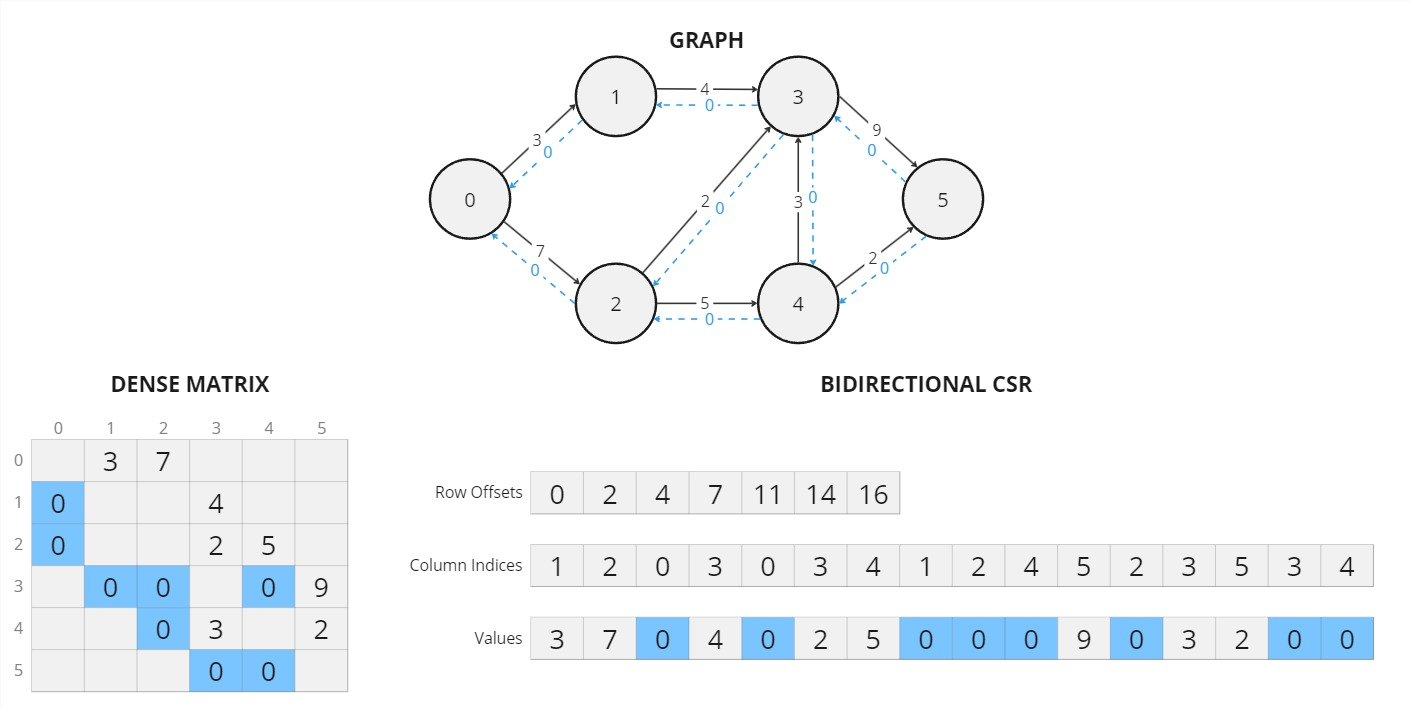
\includegraphics[width=1\linewidth]{images/bcsr-example.jpg}
                \caption{Matrice di adiacenza vs BCSR}
                \label{fig:BCSR-example}
            \end{figure}


            

        \subsection{Modifiche al codice}

            Con l'introduzione della nuova modalità di rappresentazione dei grafi, per adattare il codice della prima versione parallela, è stato sufficiente apportare delle piccole modifiche alle porzioni di codice che eseguivano accessi ai dati del grafo. Ad esempio, nei Listati \ref{code:matrix} e \ref{code:bcsr} sono confrontati gli accessi ai dati nella prima versione e quello nella seconda.
            
            \begin{listing}[h]
            \caption{Ricerca nodo vicino con matrice d'adiacenza}\label{code:matrix}
                \begin{minted}[linenos, numbersep=4pt, frame=leftline, framesep=8pt, bgcolor=bg]{cpp}
// Ricerca nodo adiacente con altezza minore
for(v = 0; v < V; v++){
    if(d_residual[u*V + v] > 0){
        h2 = d_height[v];
        ...
    }
}
                \end{minted}
            \end{listing}
            
            \begin{listing}[h]
                \caption{Ricerca nodo vicino con BCSR}\label{code:bcsr}
                \begin{minted}[linenos, numbersep=4pt, frame=leftline, framesep=8pt, bgcolor=bg]{cpp}
// Ricerca nodo adiacente con altezza minore
for(int i = d_offset[u]; i < d_offset[u+1]; i++){
    v = d_column[i];
    if(d_residual[i] > 0){
        h2 = d_height[v];
        ...
    }   
}
                \end{minted}
            \end{listing}

            Inoltre, dato che con BCSR trovare l'arco all'indietro non è immediato come nel caso con matrice di adiacenza, è stato necessario implementare un processo di ricerca apposito. Una prima soluzione è quella mostrata nel Listato \ref{code:linear-search}: per trovare l'arco all'indietro $(minV,u)$ occorre controllare per ogni vicino di $minV$ se quest'ultimo è $u$, in questo caso si salva l'indice $j$ dell'arco ricercato.
            
            \begin{listing}[h]
                \begin{minted}[linenos, numbersep=4pt, frame=leftline, framesep=8pt, bgcolor=bg]{cpp}
int backwardIdx = -1;

// Ricerca arco di ritorno
for(int j = d_offset[minV]; j < d_offset[minV+1]; j++){
    if(d_column[j] == u){
        backwardIdx = j;
        break;
    }
}
                \end{minted}
                \caption{Ricerca lineare}\label{code:linear-search}
            \end{listing}
            
            Successivamente, per sfruttare tutti i vantaggi che la BCSR offre, abbiamo sostituito questa porzione di codice con una equivalente che implementa la ricerca binaria (Listato \ref{code:binary-search}).
            
            \begin{listing}[ht]
                \begin{minted}[linenos, numbersep=4pt, frame=leftline, framesep=8pt, bgcolor=bg]{cpp}
int backwardIdx = -1;

// Ricerca arco di ritorno usando la ricerca binaria
int left = d_offset[minV];
int right = d_offset[minV + 1] - 1;

while (left <= right) {
    int mid = left + (right - left) / 2;
    if (d_column[mid] == u) {
        backwardIdx = mid;  // Arco di ritorno trovato
        break;
    } else if (d_column[mid] < u) {
        left = mid + 1;     // Cerca nella parte destra
    } else {
        right = mid - 1;    // Cerca nella parte sinistra
    }
}
                \end{minted}
                \caption{Ricerca binaria}\label{code:binary-search}
            \end{listing}
    
    \newpage
    \section{Terza versione parallela}

        Come ultima versione parallela, abbiamo voluto implementare la soluzione proposta da Hsieh et al. in \cite{EngineeringWorkload2024}. Si tratta di un approccio che combina l'utilizzo della rappresentazione BCSR e una distribuzione più equa del carico di lavoro tra i thread.

        Nelle versioni parallele analizzate finora è stato adottato un approccio \textit{thread-centric} in cui ogni thread gestiva le operazioni relative a un singolo nodo, indipendentemente dal fatto che fosse attivo o inattivo. Questo ha portato a uno spreco di risorse, poiché alcuni thread erano assegnati a nodi inattivi, mentre altri risultavano sovraccaricati, dovendo elaborare nodi con molti vicini e quindi richiedendo più lavoro.

        In questa versione si introduce, invece, un approccio \textit{vertex-centric} il quale si concentra esclusivamente sui nodi attivi distribuendo le risorse computazionali tra di essi. Hsieh et al. hanno chiamato questa versione \textit{workload-balanced push-relabel algorithm} \cite{EngineeringWorkload2024}.

        \subsection{Approccio vertex-centric}
            
            L'algoritmo inizia assegnando tutti i thread alla scansione dei vertici per individuare quelli attivi, che vengono poi aggiunti alla coda dei vertici attivi ($AVQ$). Questo approccio garantisce una distribuzione uniforme del carico di lavoro tra i thread durante la fase di identificazione dei vertici attivi. Inoltre, i vertici attivi vengono raggruppati all'interno dell'$AVQ$, consentendo di assegnare ad ogni nodo attivo un gruppo di thread (tile) per cercare il vicino con altezza minima. In questo modo, il tempo di ricerca viene ridotto.

            Nell'Algoritmo \ref{alg:workbalanced} è riportato lo pseudocodice che schematizza quanto appena detto. 
            
            Durante ciascuna iterazione, i vertici attivi vengono aggiunti alla coda AVQ tramite l'operazione AtomicAdd(). A questo punto, grazie all'inserimento di una sincronizzazione (grid.sync()), l'assegnazione dei thread può essere riorganizzata per ottimizzare la ricerca del vicino con altezza minima di ogni nodo attivo. Quando non ci sono più vertici attivi nella coda AVQ, il ciclo \verb|while| (Algoritmo \ref{alg:parallel-pr-kernel}) viene interrotto anticipatamente, evitando iterazioni non necessarie. Per migliorare l'efficienza, si usa un warp come tile che viene assegnato a ciascun vertice attivo per parallelizzare la ricerca del vicino minimo. La memorizzazione contigua dei vicini nella struttura BCSR permette di sfruttare la coalescenza della memoria, velocizzando il processo. Dopo aver identificato il vicino, il thread con $localIdx$ pari a 0 all'interno del warp esegue le operazioni di aggiornamento del grafo ("push" o "relabel").
            
            \begin{algorithm}
                \caption{\textit{PushRelabelKernel()}}\label{alg:workbalanced}
                \begin{algorithmic}
                    \State make a queue $avq$ empty
                    \State \Comment{Scanning active vertices}
                    \ForAll{$u \in V$}
                        \If{$e(u) > 0$ and $h(u) < |V|$}
                            \State $pos \gets$ AtomicAdd($avq, 1$)
                            \State $avq[pos] \gets u$  
                        \EndIf
                    \EndFor
                    \State grid.sync()
                    \State \Comment{Processing only active vertices}
                    \ForAll{$u \in avq$}
                        \State \Comment{Searching for min height neighbor of u}
                        \ForAll{$v \in neighbor(u)$}
                            \State $min =$ TiledSearchNeighbor()
                        \EndFor
                        \State tile.sync()
                        \State \Comment{Only one thread per tile computes push or relabel operations}
                        \If{$localIdx == 0$}
                            \If{$h(v) < h(min)$}
                                \State Push()
                            \Else
                                \State Relabel()
                            \EndIf
                        \EndIf
                    \EndFor
                \end{algorithmic}
            \end{algorithm}

            Nell'Algoritmo \ref{alg:tiled-search} viene descritto il processo di ricerca del vicino con altezza minima impiegando le tile. Si inizia con l'inizializzazione delle variabili necessarie e il calcolo del numero di iterazioni richieste per elaborare tutti i vicini del nodo utilizzando i thread contenuti nella tile. In questa fase preliminare si inizializza anche la memoria condivisa (shared memory), dove a ciascun thread viene assegnato lo spazio per tre interi: altezza, ID e indice del nodo vicino. Successivamente, per ogni iterazione prevista, si esaminano tutti i vicini, memorizzando solo le informazioni di quelli che soddisfano determinate condizioni.
            Una volta completata la scansione, viene effettuata una riduzione per ottenere le informazioni del nodo cercato. In seguito, uno dei thread della tile salva il risultato parziale prima di procedere all'iterazione successiva. Al termine di tutte le iterazioni, nelle variabili che contenevano i risultati parziali si troverà il risultato finale, che verrà infine restituito al chiamante.


            \begin{algorithm}
                \caption{\textit{TiledSearchNeighbor(tile, pos)}}\label{alg:tiled-search}
                \begin{algorithmic}
                    \State $idx \gets $ tile.thread\_rank() \Comment{thread index within the tile}
                    \State $tidx \gets threadIdx.x$ \Comment{thread index within the grid}
                    \State $u \gets avq[pos]$ \Comment{node whose neighbors will be scanned}
                    \State $degree \gets offset[u+1] - offset[u]$ \Comment{number of neighbors}
                    \State $numIters \gets \lceil degree / tileSize \rceil $
                    \State initialize variables $minH$ and $minV $ \Comment{to save intermediate and final result}
                    \State initialize shared memory variables $s\_height[tidx]$, $s\_vid[tidx]$, $s\_vidx[tidx]$
                    \For{$i = 0;$ $i < numIters;$ $i++$}
                        \State $vPos \gets offset[u] + i*tileSize + idx$
                        \State $v \gets column[vPos]$    
                        \If{$flows[vPos] > 0$ and $v \neq source$}
                            \State $s\_height[tidx] \gets d\_height[v]$
                            \State $s\_vid[tidx] \gets v$
                            \State $s\_vidx[tidx] \gets vPos$
                        \EndIf
                        \State tile.sync()
                        \State \Comment{Parallel reduction over shared memory values}
                        \For{$s = tile.size() / 2; s > 0; s >>= 1$}
                            \If{$idx < s$}
                                \If{$s\_height[tidx + s] < s\_height[tidx]$}
                                    \State $s\_height[tidx] \gets d\_height[tidx + s]$
                                    \State $s\_vid[tidx] \gets s\_vid[tidx + s]$
                                    \State $s\_vidx[tidx] \gets s\_vidx[tidx+ s]$    
                                \EndIf
                            \EndIf
                            \State tile.sync()
                        \EndFor
                        \State tile.sync()
                        \State \Comment{Only one thread updates the result of the current iteration}
                        \If{$idx == 0$}
                            \If{$minH > s\_height[tidx]$}
                                \State $minH = s\_height[tidx]$
                                \State $minV = s\_vid[tidx]$
                            \EndIf
                        \EndIf
                        \State tile.sync()
                        \State reset variables for next iteration
                        \State tile.sync()
                    \EndFor
                    \State tile.sync()
                    \State \Return $minV$
                \end{algorithmic}
            \end{algorithm}

            Un'ultima sostanziale differenza rispetto alle versioni precedenti è l'implementazione in CUDA anche della procedura di global-relabeling. La struttura del codice è molto simile a quella vista nelle precedenti versioni.     

    \newpage

    \section{Parallelizzazione ricerca del taglio minimo}

        Come anticipato nella Sezione \ref{sec:algoritmi}, al termine dell'esecuzione dell'algoritmo push-relabel, quello che si può ottenere immediatamente è il valore del massimo flusso. Per ottenere il minimum cutset, invece, occorre effettuare una visita in ampiezza (BFS) a partire da nodo pozzo (\textit{sink}). Nello specifico, l'insieme di taglio minimo sarà composto da tutti i nodi $v$ tali per cui esiste un cammino $v \xrightarrow{}^* sink$.

        Inizialmente, è stata implementata una versione seriale (\verb|findMinCutSetFromSink()|) che veniva eseguita sul grafo residuo restituito dall'algoritmo push-relabel. Durante i test, però, abbiamo riscontrato che la ricerca del minimum cutset impiegava, nel caso peggiore provato, decine di minuti rispetto ai pochi secondi impiegato da push-relabel.

        Vista tale differenza, abbiamo pensato di applicare delle ottimizzazioni tra cui la parallelizzazione tramite OpenMP. Di seguito descriveremo 3 versioni: quella seriale, quella parallela su matrice di adiacenza e quella parallela su rappresentazione BCSR.
        Ognuna di queste implementazioni è stata utilizzata assieme alle versioni opportune dell'algoritmo push-relabel.

        \subsection{Versione seriale}

            Questa versione è stata la prima implementata e quella che ha avuto le performance peggiori. Si tratta del punto di partenza da cui abbiamo sviluppato le versioni successive.
            Nel Listato \ref{code:mincut-serial} riportiamo il codice della funzione.

            \begin{listing}[ht]
            \begin{minted}[linenos, numbersep=4pt, frame=leftline, framesep=8pt, bgcolor=bg]{cpp}
std::vector<int> findMinCutSetFromSink(int V, int sink, int *offset, 
                                        int *column, int *forwardFlow){
    std::vector<int> minCutSet;
    std::queue<int> q;
    std::vector<bool> visited(V, false);

    // BFS per trovare il taglio minimo a partire dal nodo sink
    minCutSet.push_back(sink);
    q.push(sink);
    visited[sink] = true;

    while (!q.empty()) {
        int u = q.front();
        q.pop();

        // Scansione dei vicini di u che hanno flusso verso u
        for (int v = 0; v < V; v++) {
            for (int i = offset[v]; i < offset[v+1]; i++) {
                if(column[i] == u && forwardFlow[i] > 0 && !visited[v]) {
                    minCutSet.push_back(v);
                    q.push(v);
                    visited[v] = true;
                }
            }    
        }
    }

    return minCutSet;
}
            \end{minted}
            \caption{findMinCutSetFromSink - implementazione seriale}\label{code:mincut-serial}
            \end{listing}

        \subsection{Versione parallela su matrice di adiacenza}

            A partire dalla versione appena vista, abbiamo:
            \begin{itemize}
                \item sostituito la coda $q$ per memorizzare i nodi della frontiera con un vettore \textit{vertexList};
                \item distribuito i nodi della frontiera su più thread;
                \item introdotto delle strutture locali ai thread per ridurre gli accessi concorrenti;
                \item protetto la lettura dell'attributo \textit{visited} del nodo per evitare letture errate.
            \end{itemize}

            Per la distribuzione delle iterazioni del ciclo \verb|for| tra i thread, abbiamo provato diverse tecniche di schedulazione, quella migliore è risultata essere \verb|schedule(dynamic)|.

            La lettura di \verb|visited(v)| è stata inserita all'interno di una sezione critica per evitare race condition. Senza questa protezione, poteva verificarsi che un thread leggesse il valore \verb|false| per un nodo subito prima che un altro thread aggiornasse lo stesso valore a \verb|true|. Questa situazione avrebbe causato l'inserimento di duplicati dello stesso nodo nell'insieme del minimum cutset finale. La regione critica garantisce che l'accesso a \verb|visited(v)| avvenga in modo sicuro e sincronizzato tra i thread, prevenendo tali inconsistenze.
            
            Nel Listato \ref{code:mincut-parallel-adj} è riportato il codice completo.

            \begin{listing}
            \begin{minted}[linenos, numbersep=4pt, frame=leftline, framesep=8pt, bgcolor=bg]{cpp}
std::vector<int> findMinCutSetFromSinkOMP(int n, int t, int *residual){
    std::vector<int> minCutSet;
    std::vector<int> vertexList;
    std::vector<bool> visited(n, false);

    minCutSet.push_back(t);
    vertexList.push_back(t);
    visited[t] = true;

    while (!vertexList.empty()) {
        std::vector<int> newVertexList;
        
        #pragma omp parallel
        {
            std::vector<int> localVertexList;
            std::vector<int> localMinCutSet;

            #pragma omp for nowait schedule(dynamic)
            for (int i = 0; i < vertexList.size(); i++) {
                int u = vertexList[i];

                for (int v = 0; v < n; v++) {
                    bool shouldAdd = false;

                    #pragma omp critical (checkVisited)
                    {
                        if (!visited[v] && residual[v*n + u] > 0) {                         
                            visited[v] = true;
                            shouldAdd = true;
                        }
                    }

                    if(shouldAdd){
                        localMinCutSet.push_back(v);
                        localVertexList.push_back(v);
                    }
                }
            }

            #pragma omp critical (insert)
            {
                minCutSet.insert(minCutSet.end(), 
                    localMinCutSet.begin(), localMinCutSet.end());
                newVertexList.insert(newVertexList.end(), 
                    localVertexList.begin(), localVertexList.end());
            }
        }
        vertexList = newVertexList;
    }

    return minCutSet;
}
            \end{minted}
            \caption{findMinCutSetFromSinkOMP - implementazione parallela su matrice di adiacenza}\label{code:mincut-parallel-adj}
            \end{listing}
            
            
        \subsection{Versione parallela su rappresentazione BCSR}
     
            Per i dati rappresentati tramite il formato BCSR, l'approccio adottato è stato leggermente diverso. A causa della particolare struttura di questa rappresentazione, come già accennato, la ricerca dei nodi $v$, dato $u$, tali per cui esiste un arco ($v,u$) risulta più onerosa in termini computazionali rispetto al caso della matrice di adiacenza.
            
            Per ovviare a questo problema, tra le soluzioni analizzate, la più efficace è risultata essere quella illustrata nel Listato \ref{code:mincut-parallel-bcsr}. In questo caso, prima di iniziare la ricerca a partire dal \textit{sink}, viene calcolato il grafo residuo trasposto. Questo permette di evitare il problema della ricerca degli archi entranti, poiché una volta trasposto il grafo, sarà sufficiente seguire gli archi uscenti da ogni nodo incontrato durante la visita. 
            
            A parte questa modifica, il resto della procedura segue la stessa logica della versione basata sulla matrice di adiacenza, con alcuni adattamenti necessari per gestire la lettura dei dati secondo la struttura del formato BCSR.
            

        \begin{listing}
        \begin{minted}[linenos, numbersep=4pt, frame=leftline, framesep=8pt, bgcolor=bg, fontsize=\small]{cpp}
std::vector<int> findMinCutSetFromSinkOMP(int V, int E, int sink, 
                                int *offset, int *column, int *forwardFlow){
    int *t_offset = (int*)malloc((V+1)*sizeof(int));
    int *t_column = (int*)malloc(E*sizeof(int));
    int *t_forwardFlow = (int*)malloc(E*sizeof(int));
    for(int i = 0; i < V+1; i++){
        t_offset[i] = 0;
    }
    for(int i = 0; i < E; i++){
        t_column[i]= 0;
        t_forwardFlow[i] = 0;
    }
    
    computeTranspose(V, E, offset, column, forwardFlow, t_offset, 
                        t_column, t_forwardFlow);
    
    std::vector<int> minCutSet;
    std::vector<int> vertexList;
    bool *visited = (bool*)malloc(V*sizeof(bool));
    for(int i = 0; i < V; i++) {
        visited[i] = false;
    }
    minCutSet.push_back(sink);
    vertexList.push_back(sink);
    visited[sink] = true;
    while (!vertexList.empty()) {
        std::vector<int> newVertexList;      
        #pragma omp parallel
        {
            std::vector<int> localVertexList;
            std::vector<int> localMinCutSet;   
            #pragma omp for nowait schedule(dynamic)
            for (int i = 0; i < vertexList.size(); i++) {
                int u = vertexList[i];            
                for (int j = t_offset[u]; j < t_offset[u+1]; j++) {
                    int v = t_column[j];
                    bool shouldAdd = false;
                    #pragma omp critical (checkVisited)
                    {
                        if(!visited[v] && t_forwardFlow[j] > 0) {
                            visited[v] = true;
                            shouldAdd = true;
                        }
                    }   
                    if(shouldAdd) {
                        localMinCutSet.push_back(v);
                        localVertexList.push_back(v);
                    }
                }
            }
            #pragma omp critical (insert)
            {
                minCutSet.insert(minCutSet.end(), 
                        localMinCutSet.begin(), localMinCutSet.end());
                newVertexList.insert(newVertexList.end(), 
                        localVertexList.begin(), localVertexList.end());
            }
        }
        vertexList = newVertexList;
    }
    return minCutSet;
}
        \end{minted}
        \caption{findMinCutSetFromSinkOMP - implementazione parallela su rappresentazione BCSR}\label{code:mincut-parallel-bcsr}
        \end{listing}
    
    \newpage
    
    \section{Test e analisi delle performance}

        In ogni fase dello sviluppo delle varie versioni sono stati condotti dei test per verificare la correttezza del codice, individuare le parti da ottimizzare e confrontare le versioni finali per decretarne la migliore.
        In questa sezione descriveremo i dati utilizzati come input, le tecniche di misurazione dei tempi di esecuzione e gli strumenti per la visualizzazione dei dati ottenuti.

        \subsection{Dati di input}

            Durante lo svolgimento dei test sono stati impiegati 3 diversi gruppi di istanze di grafi:
            \begin{itemize}
                \item grafi generati casualmente con numero di nodi crescente e densità costante per misurare i tempi di esecuzione all'aumentare della dimensione dell'input;
                \item grafi generati casualmente con numero di nodi costante e densità crescente per confrontare le performance dei due tipi di rappresentazione dei grafi;
                \item grafi reperiti da un dataset online per testare gli algoritmi su istanza reali.
            \end{itemize}

            \subsubsection*{Generazione grafi casuali}

                Per la generazione dei grafi casuali abbiamo scritto un breve jupyter notebook in python e sfruttato alcune funzionalità della libreria \textit{networkx}.
                In particolare, è stata implementata la funzione \verb|generate_random_graph| (Listato \ref{code:generate-random-graph}), la quale utilizza il modello di grafi casuali Erdős-Rényi con una probabilità \textit{p} di creare un arco tra ciascuna coppia di nodi. I parametri di input per la funzione includono:
                \begin{itemize}
                    \item \verb|n|, il numero di nodi nel grafo;
                    \item \verb|p|, la probabilità con cui ogni arco viene creato tra due nodi;
                    \item \verb|min_capacity| e \verb|max_capacity|, i limiti inferiore e superiore per la capacità degli archi;
                    \item \verb|directed|, un parametro booleano che determina se il grafo sarà diretto o non diretto.
                \end{itemize}
                
                L'esecuzione della funzione genera un grafo con capacità casuali assegnate ad ogni arco. Un aspetto cruciale della generazione dei grafi è la connettività: per ogni istanza generata ci siamo assicurati che fosse connessa.
                
                Per il primo gruppo di grafi (nodi crescenti e densità costante) come valore di densità abbiamo scelto $p = 2(log(n)/n)$ poiché, secondo la teoria, la probabilità che un Erdős-Rényi random graph sia connesso è molto alta quando $p > log(n)/n$.

                Per il secondo gruppo, invece, i valori scelti sono stati $n = 1000$ e $p \in [0,1]$ con passo $0.1$.

                \begin{listing}[ht]
                \begin{minted}[linenos, numbersep=4pt, frame=leftline, framesep=8pt, bgcolor=bg]{python}
def generate_random_graph(n, p, min_capacity, max_capacity, directed=False):
    G = nx.gnp_random_graph(n, p, directed=directed, seed=7)

    for edge in G.edges:
        capacity = random.randint(min_capacity, max_capacity)
        G.edges[edge]['capacity'] = capacity
    
    return G
                \end{minted}
                \caption{Funzione per generare un grafo casuale con il modello Erdős-Rényi}\label{code:generate-random-graph}
                \end{listing}

                Una volta ottenuto il grafo generato, abbiamo scelto di salvarlo in un file di testo seguendo il formato:
                \begin{itemize}
                    \item una riga per indicare il numero di nodi presenti (es. \verb|n 500| indica 500 nodi con ID da 0 a 499);
                    \item una riga per ogni arco e la relativa capacità (es. \verb|e 1 2 5| indica arco da nodo 1 a nodo 2 con capacità 5).
                \end{itemize}
            

            \subsubsection*{Grafi da dataset online}

                I dati relativi al terzo gruppo di istanze è stato reperito al link \url{https://vision.cs.uwaterloo.ca/data/maxflow}. Si tratta di una pagina web in cui sono presenti molte istanze di grafi pesati raggruppati in dataset. Il dataset che abbiamo utilizzato per i test è chiamato \textit{BVZ-tsukuba}.

                I grafi sono salvati nel formato standard DIMACS, una sua descrizione è reperibile alla pagina \url{https://lpsolve.sourceforge.net/5.5/DIMACS_maxf.htm}.


            \subsubsection*{Lettura grafi da file}

                Come si può evincere da quanto appena detto, essendo presenti due formati di file in input, è stato necessario implementare anche due funzioni C++ per il caricamento dei dati prima dell'esecuzione dell'algoritmo push-relabel.

                La scelta di quale metodo chiamare è fatta in automatico sulla base dell'estensione del file passato al programma. Infatti, i grafi generati casualmente sono salvati in file \verb|.txt| mentre i file in formato DIMACS hanno estensione \verb|.max|.

            
        \subsection{Misurazione tempi}

            Per tutte le versioni dell'algoritmo implementate abbiamo misurato il tempo di inizializzazione (creazione e popolamento delle strutture dati e eventuali trasferimenti al device), tempo di esecuzione (dell'intero algoritmo push-relabel) e tempo totale (somma dei precedenti).

            \subsubsection*{Versione seriale}
            
                Nella implementazione seriale, per la rilevazione dei tempi, abbiamo utilizzato le funzioni della libreria \verb|chrono|. Nel Listato \ref{code:tempi-seriali} è riportato uno schema semplificato di come la misurazione è avvenuta.

                \begin{listing}[ht]
                \begin{minted}[linenos, numbersep=4pt, frame=leftline, framesep=8pt, bgcolor=bg]{cpp}
const auto start = chrono::high_resolution_clock::now();

[inizializzazione]

const auto endInitialization = chrono::high_resolution_clock::now();

[Esecuzione algoritmo push-relabel]

const auto end = chrono::high_resolution_clock::now();

double initializationTime = chrono::duration_cast<chrono::microseconds>
                                (endInitialization - start).count()/1000.0;
double executionTime = chrono::duration_cast<chrono::microseconds>
                                (end - endInitialization).count()/1000.0;
double totalTime = chrono::duration_cast<chrono::microseconds>
                                (end - start).count()/1000.0;


                \end{minted}
                \caption{Schema misurazione tempi (versione seriale)}\label{code:tempi-seriali}
                \end{listing}   

            \subsubsection*{Versioni parallele}
            
                Nelle implementazioni parallele, la misurazione dei tempi è avvenuta tramite i \verb|cudaEvent|. Nel Listato \ref{code:tempi-paralleli} è riportato uno schema esemplificativo.

                \begin{listing}[ht]
                \begin{minted}[linenos, numbersep=4pt, frame=leftline, framesep=8pt, bgcolor=bg]{cpp}
//Dichiarazione degli eventi per la misurazione del tempo
cudaEvent_t startEvent, endInitializationEvent, endEvent;
cudaEventCreate(&startEvent);
cudaEventCreate(&endInitializationEvent);
cudaEventCreate(&endEvent);

...

// Primo evento per la misurazione del tempo
cudaEventRecord(startEvent, 0);

[inizializzazione]

// Secondo evento per la misurazione del tempo
cudaEventRecord(endInitializationEvent, 0);

[Esecuzione algoritmo push-relabel]

// Terzo evento per la misurazione del tempo
cudaEventRecord(endEvent, 0);

// Attendo la fine dell'evento endEvent
cudaEventSynchronize(endEvent);

// Misurazione del tempo
float initializationTime = 0.0f;
float executionTime = 0.0f;
float totalTime = 0.0f;
cudaEventElapsedTime(&initializationTime, startEvent, endInitializationEvent);
cudaEventElapsedTime(&executionTime, endInitializationEvent, endEvent);
cudaEventElapsedTime(&totalTime, startEvent, endEvent);

// Distruzione degli eventi
cudaEventDestroy(startEvent);
cudaEventDestroy(endInitializationEvent);
cudaEventDestroy(endEvent);
                \end{minted}
                \caption{Schema misurazione tempi (versione parallela)}\label{code:tempi-paralleli}
                \end{listing}            

    \newpage
     
    \subsection{Esecuzione e analisi}

        Tutti i test eseguiti hanno prodotto dei risultati che sono stati salvati in opportuni file in formato JSON.
        Ognuno di essi conteneva:
        \begin{itemize}
            \item valore del massimo flusso;
            \item insieme dei nodi del minimum cutset;
            \item tempo di inizializzazione;
            \item tempo di esecuzione;
            \item tempo totale;
            \item numero di nodi del grafo;
            \item numero di archi.
        \end{itemize}

        Tutti questi file sono stati poi analizzati tramite un jupyter notebook in python per generare dei grafici che saranno mostrati nel Capitolo \ref{chap:Risultati}.

        Per garantire risultati più affidabili ed eliminare possibili interferenze che avrebbero potuto influenzare i risultati, ciascun test è stato eseguito 10 volte e successivamente è stata calcolata la media dei tempi registrati. 
        
        Inoltre, tutte le sessioni di test sono avvenute sulla macchina \textit{CUDA-srv} messa a disposizione dall'università con le seguenti caratteristiche:
        \begin{itemize}
            \item Intel Xeon W-3323 CPU @ 3.50GHz
            \item RAM 64GB
            \item Nvidia GeForce RTX 2080 Ti
        \end{itemize}

